% arXiv preprint. Compile with pdflatex + bibtex (or `tectonic main.tex`).
\documentclass[11pt,letterpaper]{article}

\usepackage[margin=1in]{geometry}
\usepackage[T1]{fontenc}
\usepackage[utf8]{inputenc}
\usepackage{lmodern}
\usepackage{microtype}
\usepackage{amsmath,amssymb}
\usepackage{booktabs}
\usepackage{graphicx}
\usepackage{xcolor}
\usepackage{caption}
\usepackage{tikz}
\usetikzlibrary{arrows.meta,positioning,fit,calc}
\usepackage[numbers,sort&compress]{natbib}
\usepackage{authblk}
\usepackage{enumitem}
\usepackage[hyphens]{url}
\usepackage[hidelinks,breaklinks]{hyperref}

\captionsetup{font=small,labelfont=bf}
\setlist{nosep}
\renewcommand\Authfont{\normalsize}
\renewcommand\Affilfont{\small\itshape}

\newcommand{\pkg}[1]{\texttt{#1}}
\newcommand{\mmHg}{\mathrm{mmHg}}
\newcommand{\mL}{\mathrm{mL}}

\title{\textbf{Ontology-Guided, Verifiable In-Silico Experiments on Lumped-Parameter Cardiovascular Models:\\ Semantic Connection Checking, SHACL Validation and a Receipt-Verified Language-Model Agent}}

\author[1]{Sungyeob Lim}
\affil[1]{College of Medicine, Soonchunhyang University, Republic of Korea}

\date{November 2026 \\ \small Preprint, version 1}

\begin{document}
\maketitle

\begin{abstract}
Composing physiological models from independently built components fails most often not at the equations but at the joints: two variables with the same unit can carry different meanings, metadata can be correct while the attached numbers are wrong, and a language model that is allowed to write the report can state results the engine never computed. We present an open research framework that treats each of these failure modes as a separate, testable problem. The numerical core is a deterministic closed-loop six-compartment cardiovascular model (time-varying elastance ventricles, four ideal-diode valves, linear vascular compliances) integrated as a hybrid system of smooth valve regimes joined by terminal pressure-gap events, with runtime audits of volume conservation, positivity, valve directionality and beat-to-beat settling. A semantic layer annotates 34 engine variables with label-checked Ontology of Physics for Biology (OPB) properties and Uberon/FMA anatomy, exports named-graph RDF that keeps verified labels apart from project assertions, and exposes a fail-closed connection validator that requires exact agreement of property, anatomy, bearer, reference, temporal context and flow orientation before a numeric value is transferred with an explicit unit conversion. A 12-fixture synthetic fault-injection benchmark shows the validator rejecting eight of nine unsafe connections that a scripted unguarded baseline accepts, while deliberately retaining its blind spot: correct left-ventricular metadata attached to right-ventricular data is accepted, with a maximum error of 129.8\,mmHg. An evidence-first review of the Smith et al.\ (2004) CellML model produced a 76-variable/32-equation dictionary, a 31-node anatomical specification, SHACL shapes for OMEX-metadata-style composite annotations, and a PROV-O record of reference runs; applied to the published SemSim annotation of that model, the shapes report 22 violations, 7 warnings and 46 informational results, catching the two structural defects among four previously identified by reading and neither of the two free-text defects. On top of the engine, a tool-calling language-model agent plans baseline-versus-intervention experiments from a plain-language hypothesis under a three-layer scope guard; the model chooses only runs and metric paths, every sentence and number in the report is authored by code from retained tool receipts and re-verified, and sessions are recorded in PROV-O. In a 27-case author-written evaluation, three providers (Meta Muse Spark, OpenAI, Anthropic) each passed all cases, with all 14 out-of-scope clinical requests refused by the deterministic rule layer before any model call. All physiological parameters are exploratory; nothing here is clinically validated, and we state the claim boundaries explicitly. Code, evidence ledgers, SHACL shapes, provenance records and evaluation traces are public.
\end{abstract}

\noindent\textbf{Keywords:} lumped-parameter cardiovascular model; semantic annotation; Ontology of Physics for Biology; Uberon; SHACL; PROV-O; model composition; verification and validation; LLM agents; reproducibility

\section{Introduction}
\label{sec:intro}

Lumped-parameter (zero-dimensional) models of the circulation are small enough to understand completely and rich enough to be reused and recombined \citep{shi2011lumped,smith2004minimal}. The semantic-annotation programme of the biosimulation community---composite annotations that pair an Ontology of Physics for Biology (OPB) property with an anatomical bearer \citep{gennari2011composite,cook2013opb}, the SemSim/SemGen tooling that merges models at points of biophysical overlap \citep{neal2014reappraisal,neal2015cardiomyocyte,neal2019semgen}, and the OMEX metadata specification that standardises the vocabulary \citep{neal2020omex,gennari2021omex,neal2019harmonizing}---exists precisely so that such recombination can be checked rather than assumed.

Three failure modes, however, are not addressed by annotation alone, and each shaped the design reported here.

\begin{enumerate}[leftmargin=*]
\item \textbf{Same unit, different meaning.} A pressure in mmHg may be a chamber pressure relative to a common ground, a transmural pressure across a wall, an instantaneous value or a beat mean. Equating two such variables because their units and OPB property agree is a semantic error that dimensional analysis cannot catch.
\item \textbf{Correct metadata on the wrong numbers.} A composite annotation describes a variable; it does not see the array that is bound to it. If a right-ventricular pressure column is labelled as left-ventricular, every annotation check passes and the merged model is wrong.
\item \textbf{Narration that outruns computation.} When a language model is used to plan or report an experiment, a free-text report may contain values, directions or conclusions the simulation never produced. For a research tool this is disqualifying unless every reported statement can be traced to a machine receipt.
\end{enumerate}

This paper describes a framework, built between 2026-10-31 and 2026-11-05, that isolates each failure mode in a separately testable layer: a deterministic numerical engine with executed verification evidence (Section~\ref{sec:engine}); an offline semantic registry with a fail-closed connection validator and a fault-injection benchmark that \emph{keeps} the metadata-on-wrong-numbers failure as a documented negative result (Section~\ref{sec:semantic}); an evidence-first annotation layer for the Smith et al.\ 2004 model with SHACL shapes and PROV-O records (Section~\ref{sec:evidence}); and a language-model experiment agent whose reports are authored by code from tool receipts and verified against them (Section~\ref{sec:agent}). Throughout, every numeric threshold is either cited to a source or declared a software milestone gate, and every result is labelled with what it does and does not establish.

\paragraph{Contributions.}
\begin{itemize}[leftmargin=*]
\item A hybrid event-split integration scheme for ideal-diode valve networks that never interpolates across the $\max(\cdot,0)$ corner, with tie disambiguation at roundoff-scale pressure crossings, pulse-peak checkpoints that prevent skipped valve openings, and per-regime cumulative-flow integrals whose error control does not grow with run length.
\item An offline semantic registry and connection validator with named-graph RDF export that separates source-verified labels from project assertions, and a 12-fixture fault-injection benchmark including a retained, measured false acceptance.
\item An evidence-first annotation workflow for a published CellML model: a variable dictionary, an anatomical node specification that follows current Uberon-first practice while keeping FMA cross-references, eleven generic and seven model-specific SHACL rules with positive and negative control fixtures, and a PROV-O record of OpenCOR reference runs; the workflow surfaced a unit-label defect (kPa labels on mmHg-valued parameters) and a valve-law encoding artefact in the public model.
\item A receipt-verified experiment agent in which the language model's authority is restricted to choosing a model, parameter interventions, runs and metric paths, and a 27-case cross-provider evaluation with public traces that can be re-executed in the browser.
\item A development record in which human decisions, AI-agent implementation and cross-provider review are logged with the evidence each rests on, and in which design-only verification and validation methodologies are kept separate from executed results.
\end{itemize}

\section{Related work}
\label{sec:related}

\paragraph{Minimal closed-loop models.} The Smith et al.\ (2004) minimal haemodynamic model \citep{smith2004minimal} and its descendants \citep{paeme2011mitral,revie2013porcine,pironet2013multiscale} are the reference family for this work: six elastic chambers, ventricular interaction through a septum and pericardium, and an ``open on pressure, close on flow'' valve law with inertance. Our engine is deliberately simpler (Section~\ref{sec:engine}) and is not a replication; the Smith model enters as the subject of the semantic and verification layers, through its CellML encoding in the Physiome Model Repository \citep{lloyd2008pmr,cuellar2003cellml} and reference runs in OpenCOR \citep{garny2015opencor}.

\paragraph{Semantic annotation and composition.} Composite annotations \citep{gennari2011composite}, OPB dependency classes \citep{cook2013opb}, the modular-modelling reappraisal \citep{neal2014reappraisal}, the cardiomyocyte composition use cases \citep{neal2015cardiomyocyte}, SemGen \citep{neal2019semgen}, the harmonisation recommendations \citep{neal2019harmonizing} and the OMEX metadata specifications \citep{neal2020omex,gennari2021omex} supply the vocabulary and the grammar we check against. Neal et al.\ (2015) report that automatic overlap detection missed about half the overlaps a human expert found; our design therefore treats annotation as evidence to be validated, not as authority, and the manual comparison group we sketch (Section~\ref{sec:discussion}) gives both arms the same material. Anatomy follows the Foundational Model of Anatomy (FMA) \citep{rosse2003fma} and Uberon \citep{mungall2012uberon}; BioModels.net qualifiers \citep{courtot2011qualifiers} supply the two standard relations we use.

\paragraph{Shapes and provenance.} SHACL \citep{shacl2017} validates an RDF graph against structural shapes; PROV-O \citep{provo2013} records derivation. Neither establishes physiological validity, and we use them only for what they can do: structural conformance and traceability.

\paragraph{Verification of physiological simulators.} We follow the separation of code verification, solution verification and validation in the cardiac-modelling literature \citep{pathmanathan2013reliability,pathmanathan2014verification}, the credible-practice rules of \citet{erdemir2020credible}, and the risk-informed framing of ASME V\&V 40 \citep{asme2018vv40} as summarised in the 2023 FDA guidance \citep{fda2023credibility}. Grid-convergence reporting follows \citet{roache1994gci}; event location follows \citet{shampine2000event}; the integrator is SciPy's DOP853 \citep{hairer1993,virtanen2020scipy}. No regulatory compliance is claimed.

\paragraph{Language-model agents for experiments.} Tool-using agents have planned and executed laboratory chemistry \citep{boiko2023autonomous,bran2024chemcrow}. Our contribution is narrower and about trust: the model's authority is reduced to choices that are checkable against receipts, and the report is written by code.

\section{Numerical engine}
\label{sec:engine}

\subsection{Model}

The engine (\pkg{physiosim}, Python 3.11, NumPy, SciPy) integrates six total compartment volumes $V_i$ in mL, ordered $(\mathrm{lv},\mathrm{sa},\mathrm{sv},\mathrm{rv},\mathrm{pa},\mathrm{pv})$ for left ventricle, systemic arteries, systemic veins, right ventricle, pulmonary arteries and pulmonary veins. The circulation is a directed ring
\[
\mathrm{lv}\xrightarrow{\text{aortic}}\mathrm{sa}\xrightarrow{\text{systemic}}\mathrm{sv}\xrightarrow{\text{tricuspid}}\mathrm{rv}\xrightarrow{\text{pulm.\ valve}}\mathrm{pa}\xrightarrow{\text{pulmonary}}\mathrm{pv}\xrightarrow{\text{mitral}}\mathrm{lv}.
\]
With period $T=60/\mathrm{HR}$, phase $\phi=(t \bmod T)/T$ and systolic fraction $s$, both ventricles share a cosine activation
\begin{equation}
a(\phi)=\tfrac12\bigl(1-\cos(2\pi\phi/s)\bigr)\ \text{for } 0\le\phi<s,\qquad a(\phi)=0 \text{ otherwise},
\end{equation}
so that the time-varying elastance \citep{suga1973elastance} is $E_v(t)=E_{\min,v}+(E_{\max,v}-E_{\min,v})\,a(\phi)$ for $v\in\{\mathrm{lv},\mathrm{rv}\}$. Pressures are linear in stressed volume, $P_v=E_v(t)(V_v-V_{0,v})$ for the ventricles and $P_i=(V_i-V_{0,i})/C_i$ for the four vessels, relative to one fixed external pressure of zero. Each ring edge $k$ carries $q_k=(P_k-P_{k+1 \bmod 6})/R_k$; the four valve edges are ideal diodes, $q_k:=\max(q_k,0)$, and the two vascular beds are signed resistors. Mass balance is $\dot V_i=q_{i-1}-q_i$, so $\sum_i \dot V_i\equiv 0$ symbolically; numerically, volumes are never renormalised or clipped. The model omits atria, septal and pericardial interaction, intrathoracic pressure, valve inertia, nonlinear passive mechanics, reflexes, respiration and renal regulation. All eighteen parameter defaults are author-selected exploratory values (e.g.\ $E_{\max,\mathrm{lv}}=2.5\,\mmHg/\mL$, $R_{\mathrm{systemic}}=1\,\mmHg\,\mathrm{s}/\mL$, total volume 5000\,mL), none fitted to data; the resulting baseline is an \emph{elevated-pressure} computational reference and is never described as a healthy adult.

\subsection{Hybrid event-split integration}
\label{sec:hybrid}

The right-hand side with clipped valve flows is continuous but has kinks on the surfaces $P_k=P_{k+1}$. A high-order one-step method that steps across a kink loses local order, and dense-output interpolants that span both sides of the corner can produce non-monotone cumulative valve flows. The integrator therefore solves a hybrid system: within a fixed valve regime (each valve labelled open or closed) the regime right-hand side is smooth, and each valve has a terminal event on its signed pressure gap, with direction $-1$ for an open valve and $+1$ for a closed one. Only the trajectory up to the first located root is retained; the next solve begins in the new regime. Integration also restarts at the activation boundaries $sT/2$, $sT$ and $T$ of each beat; the pulse-peak checkpoint matters because a long closed-valve step can otherwise begin and end with a negative gap while skipping an entire intervening opening and closure.

At roundoff-scale ties a short forward-Euler probe, of length $\sqrt{\varepsilon}\,T$ or half the remaining interval, whichever is smaller, chooses the right-hand regime without advancing the state; the tie resolution combines pressure-arithmetic roundoff with a few ulps of event-time error multiplied by the estimated gap slope. An exactly zero gap returns a signed $\pm\varepsilon$ sentinel so that zero-flow equilibria do not re-trigger the same event; more than eight consecutive zero-length events raise an error rather than silently skipping time. Reported flows are recomputed from the sampled pressures with the exact clipped law, so an output never shows a regime-dependent approximation.

Optionally the solver augments the state with six per-edge cumulative flows $C_k(t)=\int_0^t q_k\,dt'$. Each regime restarts its six integrals at zero and the endpoint increments are added to running offsets, so the solver's RMS error norm controls local increments rather than an ever-growing integral; the same scalar absolute tolerance in mL applies to all twelve states. Because Runge--Kutta methods preserve linear invariants and $\dot V$ and $\dot C$ are built from the same evaluated flow vector, the local balance residual $V_i-V_i(0)-(C_{\mathrm{in}}-C_{\mathrm{out}})$ stays at roundoff ($\sim\varepsilon|C|$) and verifies incidence wiring only; cumulative-flow accuracy must be shown separately by tolerance refinement. Both points were established by an independent review before the event-splitting design and are stated in the documentation and code.

\subsection{Executed verification}
\label{sec:verification}

Three canonical scenarios (baseline; reduced contractility, $E_{\max,\mathrm{lv}}$ halved; partial restoration, the impaired value $\times 1.5$) run for 60 beats at 400 samples per beat with DOP853, $\mathrm{rtol}=10^{-9}$, $\mathrm{atol}=10^{-10}$\,mL and maximum step $T/200$. Each is a separate run from identical initial volumes, not a timed treatment sequence. A runtime audit requires finite trajectories, strictly increasing time, positive volumes, no reverse valve flow and total-volume drift below $10^{-6}$\,mL; the declared milestone periodicity gate is a maximum last-versus-prior-beat six-volume waveform difference of 0.1\,mL. These are software gates, chosen before the runs; passing them is not biological validation.

An independent reviewer, working from an explicit signed incidence matrix rather than the production \pkg{np.roll} assembly, re-derived pressures, flows and derivatives on 80 seeded random states, rejected sign, scaling, source and endpoint mutations, checked each valve law at gradients of $\pm100$, $\pm10^{-9}$ and 0\,mmHg, verified unit covariance of the production routines under Pint-scaled parameters (mL$\to$L, mmHg$\to$Pa) with a corrected negative control, and compared an exact two-reservoir decay $\Delta P(t)=\Delta P(0)\exp[-t(1/C_{\mathrm{sa}}+1/C_{\mathrm{sv}})/R_{\mathrm{sys}}]$ against the production six-state model under step refinement. A coupled tolerance/step ladder (default $10^{-7}/10^{-8}/T{/}100$; tight $10^{-9}/10^{-10}/T{/}200$; fine $10^{-11}/10^{-12}/T{/}400$) quantified refinement differences. Separately, the package was built as a wheel, installed in a clean environment and executed twice in isolated mode; the three numerical CSVs were byte-identical and the parsed summaries equal (same-host determinism, not cross-platform identity).

\section{Semantic registry, connection validation and fault injection}
\label{sec:semantic}

\subsection{Registry and RDF export}

\pkg{physiosim.ontology} is an entirely offline registry of 34 engine variables: six pressures, six volumes, two ventricular elastances, four compliances, six directed flows, six resistances, heart rate, cardiac output, stroke volume and total volume. Each entry records physical property, anatomical context, physical bearer, temporal context (instantaneous, complete-beat mean, complete-beat integral), unit, pressure reference, flow orientation, the governing equation string, dependencies and a source document pointer. Six OPB properties are label-checked against a pinned OPB v1.07 file (fluid pressure, fluid volume, fluid flow rate, fluid flow resistance, fluid volumetric elastance, event frequency). Anatomy follows the node specification of Section~\ref{sec:nodes}: ten nodes with a Uberon primary identifier and the FMA cross-reference retained (blood, the two ventricular cavities, the four valves, the heart and the two ventricles). Left- and right-ventricular pressure and volume are properties of blood that is \pkg{bqbiol:isPartOf} the ventricular cavity; the four valve flows carry \pkg{bqbiol:occursIn} their valve \citep{courtot2011qualifiers}. The lumped systemic and pulmonary compartments, cardiac output and stroke volume are explicitly \emph{local} concepts in a project namespace, because no recorded decision maps them to a named vessel lumen.

The export is an RDF dataset with three named graphs: verified external labels and cross-references; project model assertions; and a provenance graph stating the status of each. No \pkg{owl:sameAs}, \pkg{owl:equivalentClass}, subclass or disease-diagnosis triple is manufactured, and flattening serialisations are refused so that graph boundaries cannot silently disappear.

\subsection{Connection validator}

\pkg{validate\_connection(source, target, conversion)} either returns an immutable connection whose \pkg{convert} method applies the required numeric factor, or raises. It first rejects empty required descriptors and unknown flow endpoints, then requires exact equality of anatomy and property identifiers, flow location, bearer kind, biological and temporal context, pressure reference and orientation, then checks each endpoint's unit against the property's unit contract, and finally requires an explicit \pkg{UnitConversion} whenever the two unit strings differ, even for Pint aliases; Pint computes the multiplier. Unknown properties fail closed; custom factors, offsets and sign reversal are unsupported. The check establishes direct variable equivalence only: a pressure cannot be equated to a flow by relabelling units, and connecting a pressure port to a downstream port is the job of a component equation, not of the validator. \pkg{connect\_value} binds a registered name to the actual engine array or metric and applies the conversion on transfer; the canonical experiment exercises this path for cardiac output and tests that the transferred value agrees with the direct metric to roundoff.

\subsection{Synthetic fault-injection benchmark}

Twelve hand-written fixtures pair a source descriptor with a target descriptor and a ground-truth label assigned by the author, not computed by the validator. Three are correct (same pressure, same flow, explicit mmHg$\to$Pa conversion); nine are faults: wrong anatomy, wrong property, reversed flow, wrong reference, wrong temporal context, wrong dimensions, missing conversion, wrong bearer and a mis-annotated payload. Three conditions are scored: \emph{manual}, a scripted unguarded baseline that accepts every submission; \emph{units-only}, which checks dimensions and explicit scaling; and \emph{semantic}, the full validator. The mis-annotated payload fixture is executed with real arrays: the computed right-ventricular pressure column is handed over under a correct-looking left-ventricular descriptor. This is a small synthetic experiment, not a user study; human integration effort was not measured.

\section{Evidence-first annotation of the Smith 2004 model}
\label{sec:evidence}

\subsection{Sources, dictionary and licence}

Before any ontology engineering, the project obtained and read the full texts of the composite-annotation, OPB, modular-modelling, SemGen, harmonisation and OMEX papers, the three Smith-derivative papers, the two W3C Recommendations, the 2004 author manuscript (36 pages, quotations only retained), and the SemSim-annotated CellML of the Smith model in Physiome workspace 267, with each source recorded as an evidence card holding exact quotations with locations, the distinction between claim, interpretation and independent confirmation, licence and limits. A retrieval ledger records URL, method, licence and SHA-256 for every retained file. Abstract-only sources were not allowed to fix any relation direction or mapping; unsettled points are recorded as \texttt{UNKNOWN}.

Two CellML captures were compared statically: the workspace-267 SemSim copy and the canonical exposure file (changeset \texttt{f7b732c9}). Both have 14 components, 32 equations and 94 variable connections, but the SemSim copy carries no \pkg{initial\_value} attributes, so 43 parameters and 10 initial conditions are absent and it cannot be simulated as captured. A 76-variable, 32-equation dictionary was produced from the canonical file with units, role, SemSim annotation, reference point, direction and unit plausibility. Both captures fall under the Physiome Model Repository's CC BY 3.0 statement; attribution to the CellML author, the original paper and the repository is recorded.

\subsection{Findings that annotation alone could not have produced}
\label{sec:conflicts}

Eleven conflicts (C1--C11) were logged. Three are worth stating here.

\textbf{C1, unit labels.} The canonical CellML declares kPa, kPa/mL, kPa$\cdot$s/mL and kPa$\cdot$s$^2$/mL, yet the 2004 manuscript uses mmHg, mL and s throughout (26 occurrences of ``mmHg'', none of ``kPa''), Paeme et al.\ \citep{paeme2011mitral} tabulate the same numerals in mmHg-based units, the six CellML initial volumes sum exactly to the manuscript's 1500\,mL stressed volume, and the unmodified model yields an aortic pressure of 79--116 in the file's own units, matching the manuscript's target of about 120/80\,mmHg; a kPa reading would mean roughly 590--870\,mmHg. The recorded decision reads the numerals as mmHg-based and applies no factor, while recording that the manuscript tabulates no parameter values and so no individual numeral's unit is stated by its authors. Had a kPa$\to$mmHg factor of 7.5 been applied on the strength of the declared units, every cross-model comparison would have been corrupted.

\textbf{C5, bearer granularity.} The project registry had annotated $P_{\mathrm{lv}}$ to the organ ``Left ventricle'' (FMA:7101); the SemSim reference uses ``Portion of blood \emph{part\_of} Cavity of left ventricle'' (FMA:9466). Both labels verify; they are different entities. The decision adopted the blood-in-cavity form, following the composite-annotation grammar \citep{gennari2011composite}, and this was later applied to the registry.

\textbf{C11, valve-law encoding.} The manuscript implements ``close on flow, open on pressure'' by removing a flow from the state vector when it turns negative; the CellML keeps the flow as a state and sets $\dot Q=0$ while $\Delta P<0$ and $Q<0$, so a negative flow reached within one step is frozen rather than reset. OpenCOR reference runs (Section~\ref{sec:opencor}) show exactly this: three negative aortic-flow spans per run, each exactly constant, with $P_{\mathrm{lv}}-P_{\mathrm{ao}}<0$ throughout. The negative values are an artefact of the encoding, not physiology.

\subsection{Anatomical node specification v2}
\label{sec:nodes}

Every anatomical structure a variable, process or equation refers to is an explicit node, not free text. The identifier rule follows current physiology-infrastructure practice (NIH SPARC, SCKAN and the Human Reference Atlas): the Uberon term when Uberon has the same structure (matched by FMA cross-reference), otherwise the FMA term, with the other identifier recorded on every node. Uberon was released 2026-10-01 and is active; FMA 5.1.0 (2026-05-15) is listed inactive by the OBO Foundry; OMEX metadata v1.2 still recommends FMA, and this counter-evidence is recorded. The specification has 31 nodes: 27 take a Uberon primary identifier, and the four vessel-tree lumens keep FMA because Uberon has no vessel-specific lumen term. The Smith ``aorta'' and ``vena cava'' chambers are read, from the manuscript's wording that the periphery is ``modelled using elastic chambers, simulating the arteries and veins'', as the systemic arterial and venous tree lumens rather than the named vessels; the atria, which the manuscript omits ``as they contribute only minimally'', are lumped parts of the venous compartments with \pkg{bqbiol:hasPart}; the minor heart valves, venae cavae and coronary sinus are catalogue nodes with identifiers but no assertions. Both the compartment reading and the atrial lumping are recorded as interpretations.

\subsection{SHACL shapes and PROV-O}

Eleven generic rules encode the OMEX v1.2 composite-annotation structure (allowed OPB property class, bearer present, fluid-volume bearer is a fluid portion, pressures as energy differentials with source and sink, processes with participants, constitutive parameters, v2 containers, v2 valve locations, coverage), and seven Smith-specific rules encode what the equations require (chamber pressures have no sink while free-wall pressures have the pericardial contents as sink; a pressure and its volume are borne by the same blood; flow direction matches the driving pressure difference; valve flows occur in their valve; venous compartments include their atrium; each compartment lies in its v2 container). The third to fifth rules read a hand-written dependency file that the runner re-checks against the dictionary's equations. A positive-control fixture must yield zero results and two negative-control fixtures must yield exactly 13 and 12 expected results; the controls caught two defects in the first draft of the shapes (severity placed on the SPARQL constraint rather than the shape; a nested detail counted as a separate result) before the finding run. The workspace-267 SemSim RDF is mechanically translated to OMEX form, keeping every defect, and validated.

A PROV-O record \citep{provo2013} describes the OpenCOR reference runs: input file hashes, solver settings read back before and after each run, output hashes, the wrapper boundaries that are known and the times that are unknown, and the status of the solver attribution. Evidence, extracted facts, interpretations and conflicts carry separate predicates. A checker script re-resolves every referenced file.

\subsection{OpenCOR reference runs}
\label{sec:opencor}

The canonical CellML was run in OpenCOR 0.8.3 on a separate Linux host. The default configuration (CVODE with KINSOL) failed with ``the maximum number of iterations was reached before convergence''; the message names no solver, and which of CVODE or KINSOL failed is recorded as unknown rather than inferred. With user approval the fixed-step fourth-order Runge--Kutta solver replaced CVODE only, at three step sizes (A $10^{-5}$, B $5\times10^{-6}$, C $2.5\times10^{-6}$\,s) over 1.5\,s with 1\,ms output. The quantities of interest, scalar definitions, time-stamp equality bound ($|\Delta t|\le N_{\mathrm{steps}}\,\varepsilon\,t_{\max}$, derived from IEEE~754 arithmetic rather than chosen) and the decision to report without a pass/fail line were fixed before run C existed, following the position in the verification literature that no universal numeric acceptance threshold exists and the level is set by context of use \citep{pathmanathan2013reliability,pathmanathan2014verification,erdemir2020credible}.

\section{Four-chamber model and two-model contracts (candidate work)}
\label{sec:m1}

A second engine, \pkg{four\_chamber\_m1}, adds passive atria (eight volume states, order lv, sa, sv, ra, rv, pa, pv, la; four diodes and four signed resistors; constant atrial elastances) and reuses the Section~\ref{sec:hybrid} integrator with eight per-regime flow integrals. Its numerical acceptance bounds (total drift $10^{-7}$\,mL; local balance $10^{-6}$\,mL; passive matrix-exponential subproblem $10^{-6}$\,mL; DOP853 refinement $10^{-5}$\,mL; Radau versus DOP853 $10^{-4}$\,mL; large-step pulse $10^{-4}$\,mL volumes and $10^{-5}$\,mL integrals; symmetric simultaneous circuits $10^{-7}$/$10^{-6}$\,mL) were declared before implementation. The model has no parameter defaults; a synthetic fixture (5120\,mL) exists for software exercise and is labelled as such. A closed manifest validator checks the model's semantic contract against the bundled node specification and rejects reversed topology, mismatched identifiers, lumen-identity assertions and any extra field.

Three further rounds (ONTO-R1 to R3g, 2026-11-02 to 2026-11-05) generated typed model-scoped quantity contracts for every engine quantity of both models (OPB base property plus aggregation tag, bearer, process and anatomy context with usage status, evidence pointers), a unified deterministic TriG dataset (366 quantities, 325 laws including the signed incidence of the four-chamber model, 16,281 quads in named graphs), and a project SHACL profile separate from the Smith profile in which the real export conforms and 61 fixtures behave as expected (3 conform, 58 rejected), with two mutations (an incidence-sign flip and an equation-literal change) declared outside SHACL scope by design and caught instead by independent RDF-to-engine incidence tests. A lung-anatomy context (13 classes, 11 source relations, 7 atlas selector records, 84 project-authored non-identity links) was retained as context only, with every link carrying an assertion basis and licence pointer, and blood entities, compartments and quantities are forbidden from being typed as or linked directly to lung classes. The integrator's own finding in the last round is instructive: validation results had depended on hash order and run context, because \pkg{rdflib}'s list iteration followed one arbitrary branch of a branching \pkg{rdf:List} and a test helper selected named graphs by enumeration order; lists are now enumerated completely, malformed lists fail closed, and determinism tests run under several \pkg{PYTHONHASHSEED} values. These rounds are committed as candidate data for independent review and have \emph{not} been independently reviewed; the numerical engine and its fingerprint are unchanged through all of them.

\section{Receipt-verified experiment agent}
\label{sec:agent}

\begin{figure}[t]
\centering
\resizebox{\textwidth}{!}{%
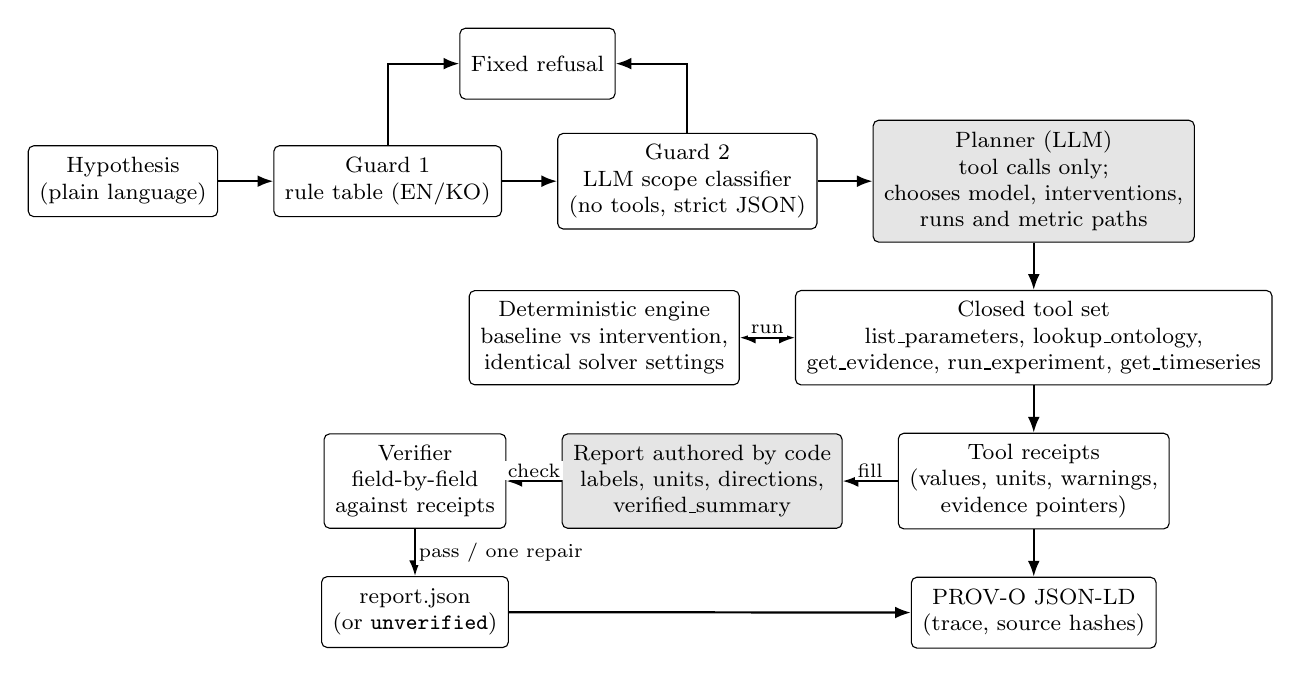
\begin{tikzpicture}[
  node distance=6mm and 7mm,
  box/.style={draw,rounded corners=2pt,align=center,font=\footnotesize,inner sep=4pt,minimum height=9mm},
  dark/.style={box,fill=black!10},
  arr/.style={-{Latex[length=2mm]},thick},
  lab/.style={font=\scriptsize,fill=white,inner sep=1pt}
]
\node[box] (h) {Hypothesis\\(plain language)};
\node[box,right=of h] (g1) {Guard 1\\rule table (EN/KO)};
\node[box,right=of g1] (g2) {Guard 2\\LLM scope classifier\\(no tools, strict JSON)};
\node[dark,right=of g2] (p) {Planner (LLM)\\tool calls only;\\chooses model, interventions,\\runs and metric paths};
\node[box,above=5mm of $(g1.north)!0.5!(g2.north)$] (ref) {Fixed refusal};
\node[box,below=of p] (t) {Closed tool set\\list\_parameters, lookup\_ontology,\\get\_evidence, run\_experiment, get\_timeseries};
\node[box,left=of t] (e) {Deterministic engine\\baseline vs intervention,\\identical solver settings};
\node[box,below=of t] (r) {Tool receipts\\(values, units, warnings,\\evidence pointers)};
\node[dark,left=of r] (c) {Report authored by code\\labels, units, directions,\\verified\_summary};
\node[box,left=of c] (v) {Verifier\\field-by-field\\against receipts};
\node[box,below=of v] (o) {report.json\\(or \texttt{unverified})};
\node[box,below=of r] (prov) {PROV-O JSON-LD\\(trace, source hashes)};
\draw[arr] (h)--(g1); \draw[arr] (g1)--(g2); \draw[arr] (g2)--(p);
\draw[arr] (g1.north)|-(ref.west);
\draw[arr] (g2.north)|-(ref.east);
\draw[arr] (p)--(t);
\draw[arr,{Latex[length=2mm]}-{Latex[length=2mm]}] (t)--(e) node[lab,midway,above]{run};
\draw[arr] (t)--(r);
\draw[arr] (r)--(c) node[lab,midway,above]{fill};
\draw[arr] (c)--(v) node[lab,midway,above]{check};
\draw[arr] (v)--(o) node[lab,midway,right]{pass / one repair};
\draw[arr] (r)--(prov);
\draw[arr] (o)--(prov);
\end{tikzpicture}}
\caption{Experiment-agent pipeline. The language model's authority is limited to the shaded boxes; every sentence and number in a report is produced by code from receipts and re-verified. Free model text is never stored; only its SHA-256 and length are kept in the trace.}
\label{fig:agent}
\end{figure}

A researcher supplies a hypothesis such as ``In M1, halve LV peak elastance and compare cardiac output.'' Figure~\ref{fig:agent} shows the pipeline. A deterministic rule table of English and Korean patterns for personal-health, diagnosis, treatment, drug and dosing requests runs before any provider is created. A one-call scope classifier using the same provider, without tools, must return a strict \texttt{\{in\_scope, reason\}} object; malformed replies, tool calls and provider errors fail closed. The planner then sees a research-only system prompt and five JSON-schema tools over the engine and the ontology; interventions are absolute values or scale factors within exploration ranges ($\times0.1$ to $\times5$ of the default, intersected with engine validity), and a baseline--intervention pair always uses identical solver settings. The final message the model may author is only \texttt{\{model, findings:[\{run\_id, metric\_path\}]\}}.

Everything else---the original hypothesis, every run's parameter changes and overrides, diagnostics, warnings and caveats, anatomical binding identifiers, relevant ontology and evidence receipts, finding values with full precision, labels, units, directions and the \texttt{verified\_summary} text---is filled in by code from the retained receipts. Directions use a tolerance of $10\,(\mathrm{atol}+\mathrm{rtol}\cdot\text{scale})$, so a change inside solver tolerance is reported as ``no meaningful change''. Model-supplied copies of these fields are discarded even when fabricated. A verifier checks each code-filled field against the session receipts and the summary by exact equality; one tool-free repair turn is allowed, after which the report becomes a minimal \texttt{unverified} envelope. Per-session limits are 180\,s wall clock, six experiments, eight ordinary model calls plus one classifier and one repair call, and at most 80 solver cycles. Each session writes a trace and a PROV-O JSON-LD record with runtime source hashes. The tool layer imports only the standard library, NumPy, SciPy and the lightweight engine modules, so the recorded sessions can be replayed and the engine re-executed in the browser through Pyodide on the public site, where every finding is re-verified against the re-run.

The evaluation suite holds 27 author-written cases: 13 in-scope experiments across both engines (mitral resistance, LV peak elastance, heart rate, systemic and pulmonary resistance, arterial compliance, initial volume, review counter-examples and three formerly refused experiment phrasings) and 14 out-of-scope clinical requests, including Korean ones, that must be refused. Expected signs were obtained by executing the engine. Three providers were run once each on 2026-11-02 on the same commit.

\section{Development process}
\label{sec:process}

The code was written by AI coding agents (OpenAI Codex, Anthropic Claude) orchestrated by a routing agent under a cross-provider policy: work implemented by one provider family is reviewed by the other, and the agent module went through three such review rounds. Three role-separated workstreams supplied physiology, semantic engineering and independent verification. Decisions that needed a human---the C1 unit reading, the C5 bearer form, the pressure-reference convention, the RK4 solver deviation, the time-stamp bound and its supersession, the node specification, which relations use standard qualifiers---were made by the repository owner and recorded with date, evidence and scope in a decision log. Two methodology documents written on 2026-11-03 are design-only and are kept apart from executed results: a model-verification methodology that frames the work under ASME V\&V 10/20/40 and the FDA 2023 guidance and reports, among other findings, that the integrated system is the hybrid regime system rather than the clipped ODE the documentation originally described, that no independent (Level-3) implementation exists, and that valve event times have never been checked; and a physiological-validation methodology that fixes a context of use, pre-registers every threshold or declares the test report-only, and names candidate datasets without opening them.

\section{Results}
\label{sec:results}

\subsection{Canonical scenarios}

\begin{table}[t]
\centering\small
\caption{Final-beat metrics of the three canonical scenarios (60 beats, DOP853, rtol $10^{-9}$, atol $10^{-10}$\,mL, max step $T/200$, 400 samples/beat). Forward SV integrates aortic flow; EDV/ESV are sampled extrema; means are time-weighted. All parameters are exploratory; the baseline is an elevated-pressure computational state, not a healthy reference.}
\label{tab:scenarios}
\begin{tabular}{lrrr}
\toprule
 & Baseline & Reduced contractility & Partial restoration \\
\midrule
$E_{\max,\mathrm{lv}}$ (mmHg/mL) & 2.500 & 1.250 & 1.875 \\
Cardiac output (L/min) & 7.699 & 6.699 & 7.331 \\
Forward stroke volume (mL) & 102.66 & 89.32 & 97.75 \\
LV EDV / ESV (mL) & 177.7 / 75.1 & 214.1 / 124.7 & 190.9 / 93.1 \\
LV ejection fraction & 0.577 & 0.417 & 0.512 \\
Systemic systolic / diastolic (mmHg) & 163.0 / 104.7 & 142.8 / 91.4 & 155.7 / 99.9 \\
Systemic mean (mmHg) & 133.5 & 116.4 & 127.3 \\
Pulmonary arterial mean (mmHg) & 23.76 & 24.17 & 23.91 \\
Pulmonary venous mean (mmHg) & 10.94 & 13.00 & 11.69 \\
Max total-volume drift (mL) & $1.5\times10^{-11}$ & $2.4\times10^{-11}$ & $3.2\times10^{-11}$ \\
Last/prior-beat max difference (mL) & $2.3\times10^{-5}$ & $9.6\times10^{-6}$ & $9.3\times10^{-6}$ \\
\bottomrule
\end{tabular}
\end{table}

\begin{figure}[t]
\centering
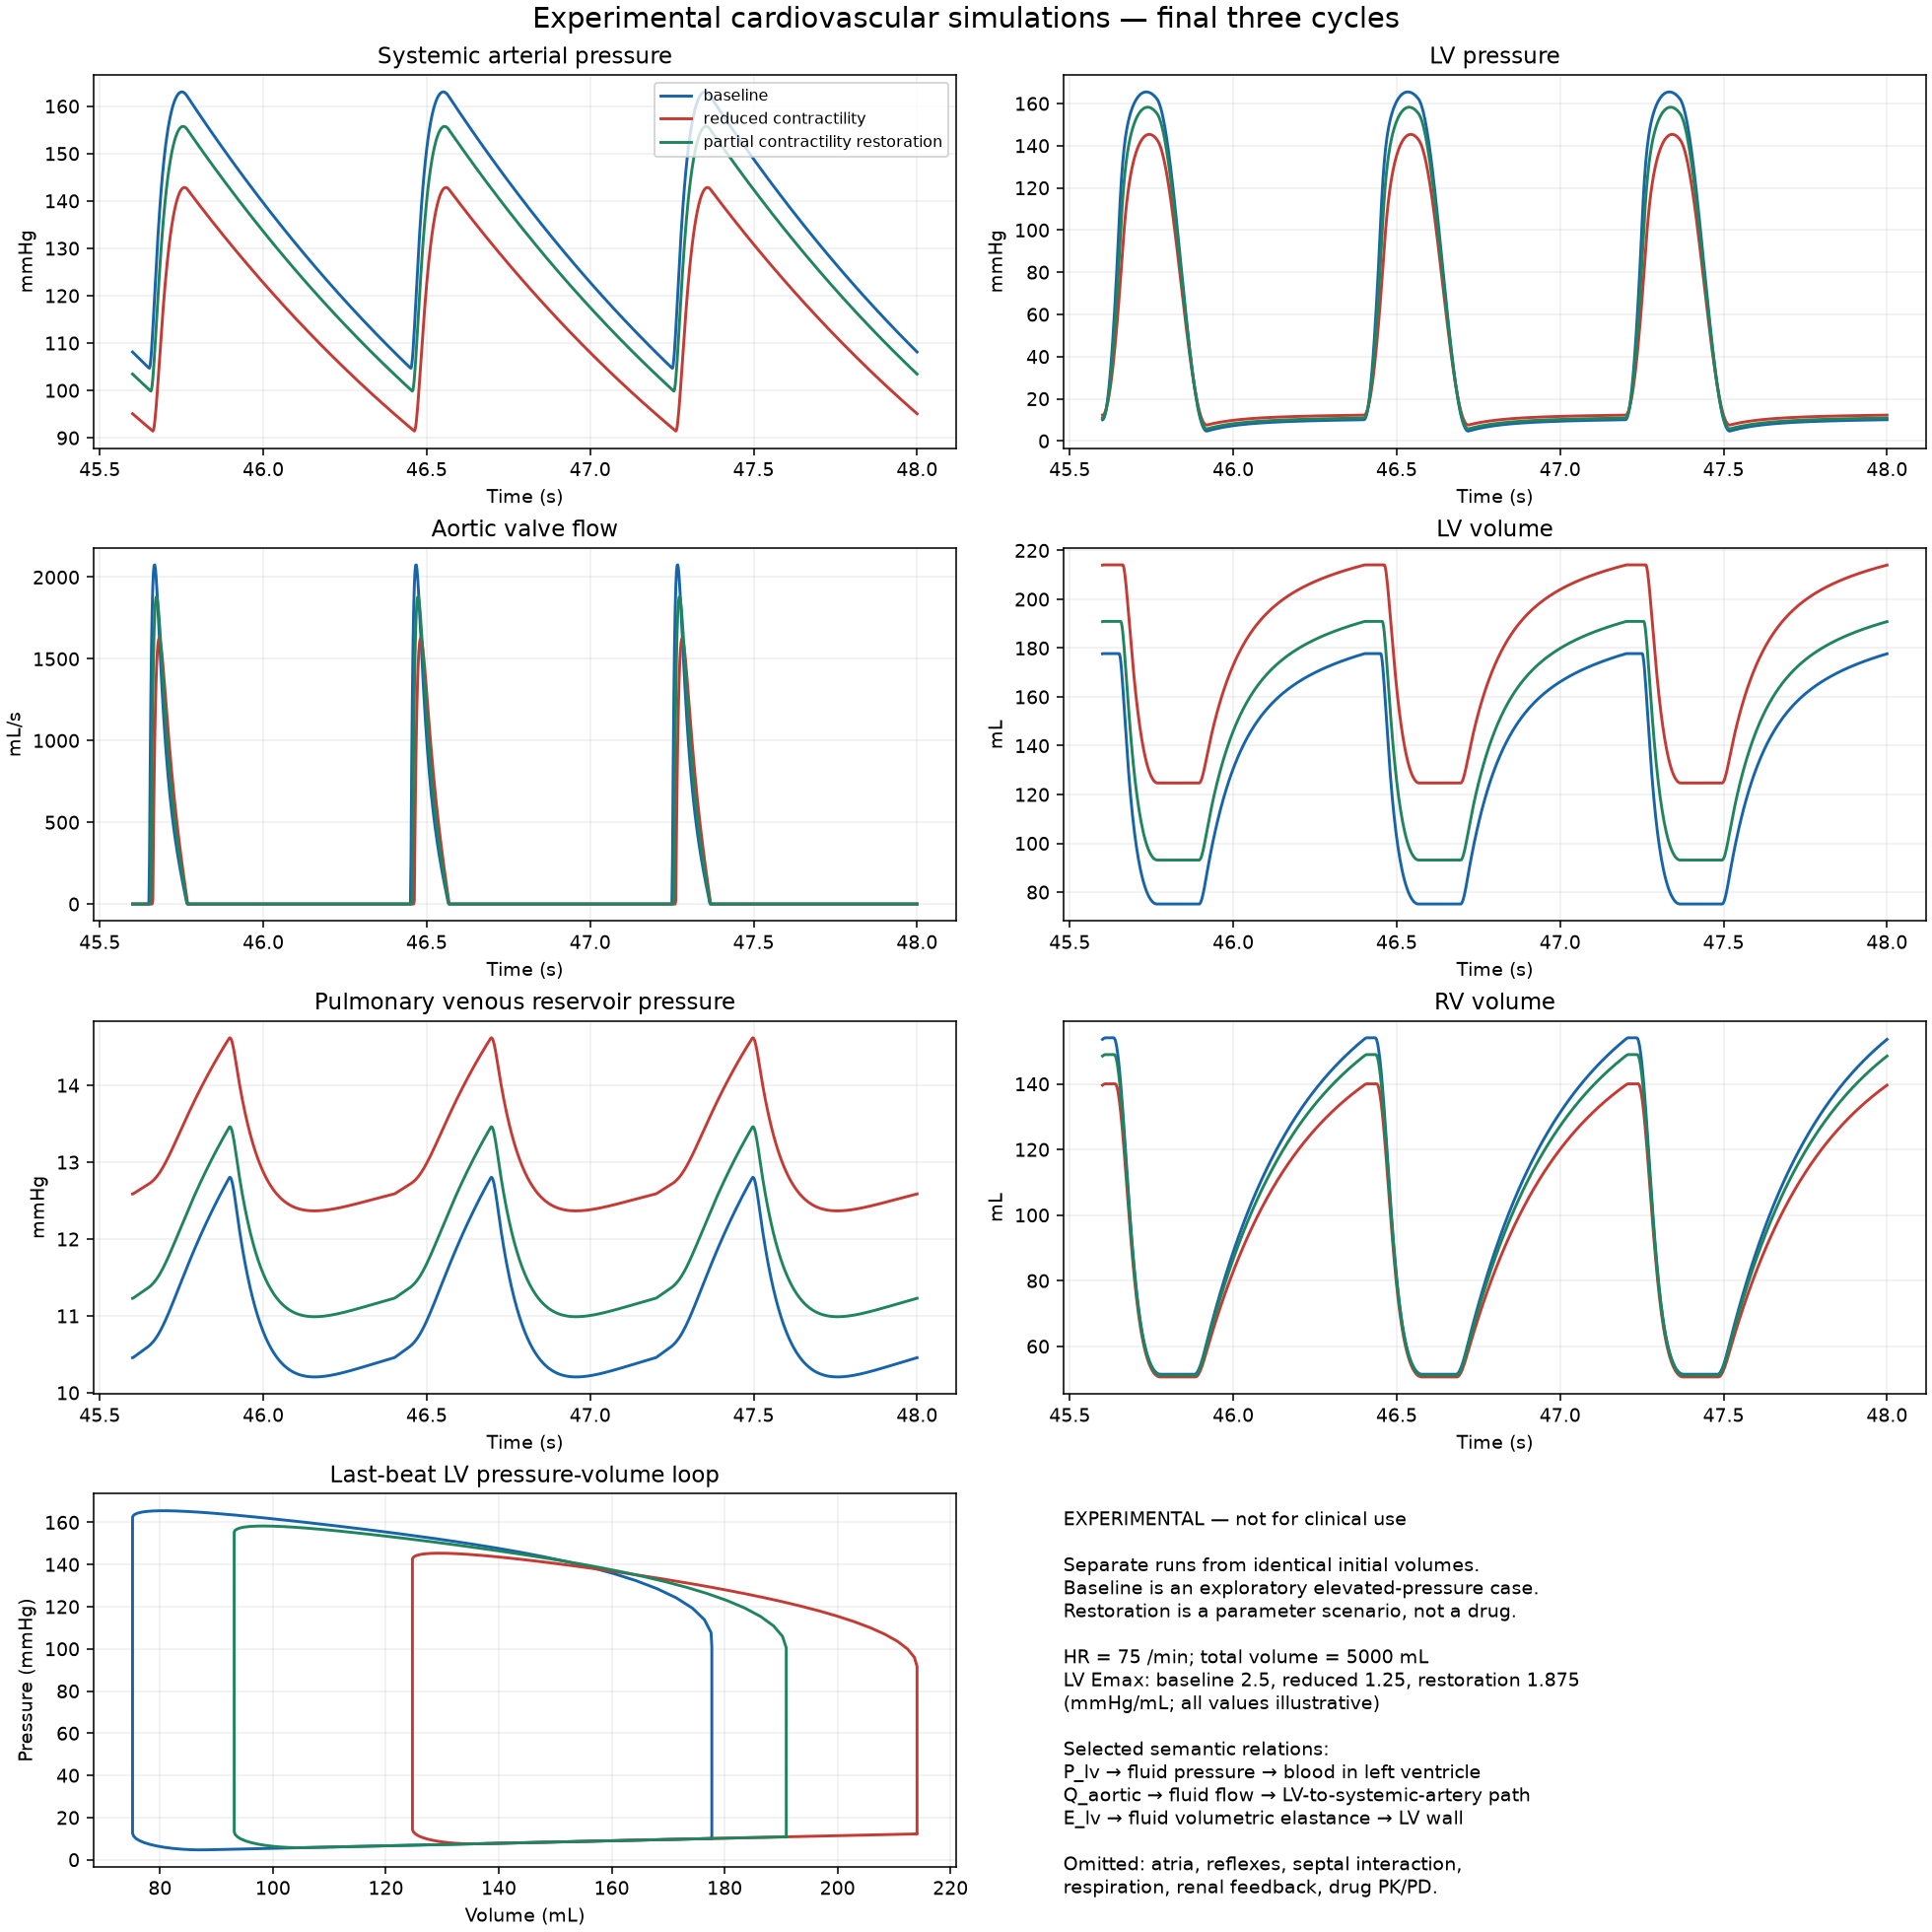
\includegraphics[width=0.78\textwidth]{figures/comparison.png}
\caption{Last three beats of the three canonical scenarios: pressures, flows, ventricular volumes and the left-ventricular pressure--volume loop, as generated by the experiment runner.}
\label{fig:comparison}
\end{figure}

\begin{figure}[t]
\centering
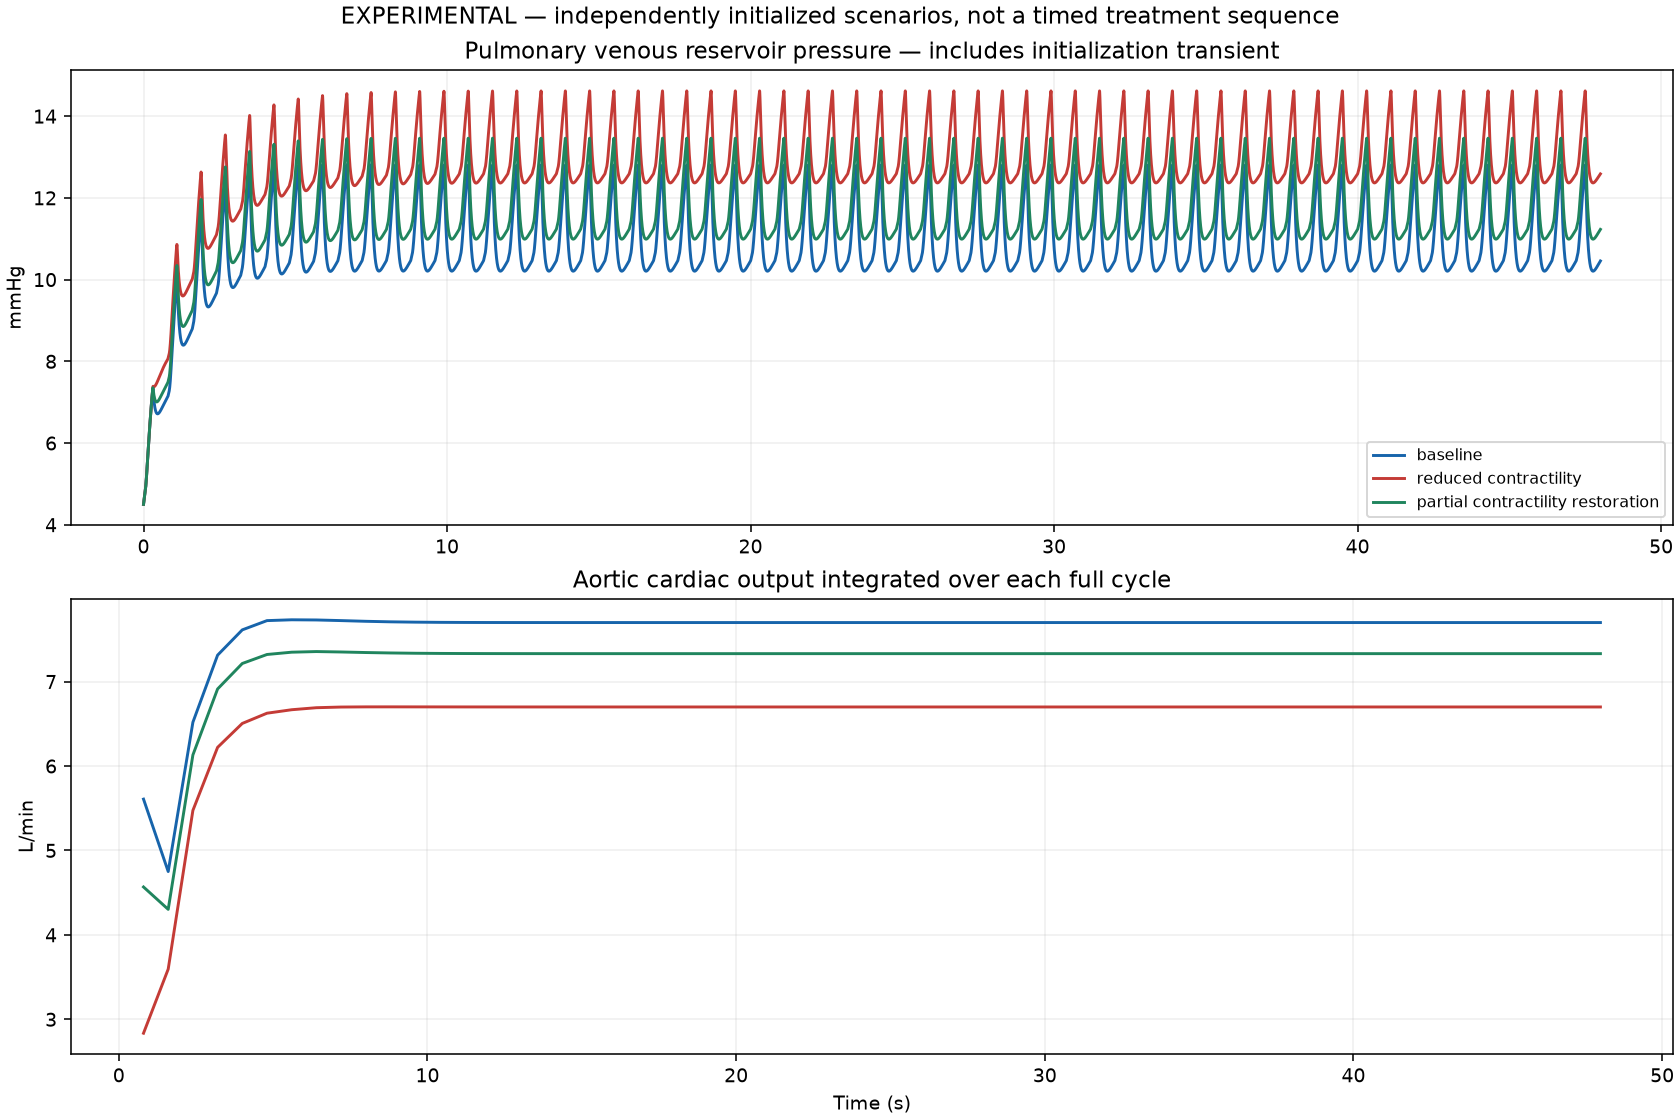
\includegraphics[width=0.78\textwidth]{figures/transients.png}
\caption{Full 60-beat runs: pulmonary venous reservoir pressure and cycle-integrated cardiac output, including the initialisation transient. The pulmonary venous pressure is a lumped reservoir pressure, not a measured atrial pressure.}
\label{fig:transients}
\end{figure}

Table~\ref{tab:scenarios} and Figures~\ref{fig:comparison}--\ref{fig:transients} summarise the canonical runs. For this parameter set, halving LV peak elastance lowered output and ejection fraction and raised end-systolic volume and pulmonary venous pressure; this is a conditional mechanistic result for this model and inventory, not a monotonicity theorem and not a heart-failure diagnosis. All three runs passed the runtime audit and the 0.1\,mL milestone gate; total-volume drift stayed at roundoff with no renormalisation.

\subsection{Numerical verification}

\begin{table}[t]
\centering\small
\caption{Recorded refinement and strict-periodicity results from the independent verification report (60 beats, both scenarios). ``Strict'' requires each of the last three beat-to-beat residuals $\le 10^{-4}$\,mL. Maximum full-trajectory volume difference: baseline default versus tight 0.3153\,mL (peaking at $t=28.9$\,s in the systemic arterial compartment); tight versus fine $1.03\times10^{-3}$\,mL. Maximum last-beat volume difference, tight versus fine: $1.74\times10^{-5}$\,mL (baseline), $8.05\times10^{-6}$\,mL (reduced).}
\label{tab:refine}
\begin{tabular}{llrrrc}
\toprule
Scenario & Settings & Beat 58 (mL) & Beat 59 & Beat 60 & Strict pass \\
\midrule
Baseline & default & $5.55\times10^{-3}$ & $2.78\times10^{-3}$ & $2.18\times10^{-3}$ & no \\
Baseline & tight & $2.33\times10^{-4}$ & $7.37\times10^{-5}$ & $2.29\times10^{-5}$ & no \\
Baseline & fine & $8.79\times10^{-7}$ & $3.55\times10^{-7}$ & $2.31\times10^{-7}$ & yes \\
Reduced & default & $2.23\times10^{-3}$ & $1.91\times10^{-3}$ & $1.98\times10^{-3}$ & no \\
Reduced & tight & $9.42\times10^{-6}$ & $7.39\times10^{-6}$ & $9.57\times10^{-6}$ & yes \\
Reduced & fine & $1.73\times10^{-7}$ & $1.51\times10^{-7}$ & $1.98\times10^{-7}$ & yes \\
\bottomrule
\end{tabular}
\end{table}

The independent oracles agreed with production on all 80 seeded states, with the largest metric discrepancy $8.9\times10^{-16}$; all mutation controls were rejected; the unit-covariance check gave trajectory errors of $8.7\times10^{-8}$\,mL and $3.5\times10^{-8}$\,mmHg; the exact reservoir decay was reproduced with errors falling $6.1\times10^{-5}\to7.3\times10^{-6}\to9.0\times10^{-7}$\,mL under step refinement. Table~\ref{tab:refine} shows that the milestone gate is comfortably met at all settings but that the strict three-beat criterion is \emph{not} met for the tight baseline: at canonical tolerances the residuals are dominated by integration error, are not monotone, and change verdict when only the error-controlled state set changes. Strict-periodicity claims therefore require the fine settings or a demonstrated refinement sequence, and the documentation says so.

Post-processing accuracy is separate from ODE accuracy. Resampling the same dense solution at 400, 800 and 1600 samples per beat changed forward stroke volume by about 0.057\% (baseline) and 0.059\% (reduced), non-monotonically because valve timing interacts with the sampling grid; trapezoidal integration on native adaptive nodes left whole-run local balance residuals of 79.9, 24.9 and 6.8\,mL at default, tight and fine settings while the state-volume drift stayed below $3.4\times10^{-11}$\,mL. These findings motivated the solver-integrated cumulative flows of Section~\ref{sec:hybrid}, whose acceptance tests require four-cycle augmented/plain volume agreement within $10^{-4}$\,mL and 40-cycle tight/fine cumulative stroke-volume agreement within $10^{-5}$\,mL with zero relative allowance. A wheel built from the repository passed 64 tests in a clean environment at the time of the canonical run; the main branch later carried 117 tests.

\subsection{Semantic benchmark}

\begin{table}[t]
\centering\small
\caption{Twelve-fixture synthetic fault-injection benchmark (3 correct, 9 faulty connections). Ground truth is author-assigned.}
\label{tab:benchmark}
\begin{tabular}{lrrrr}
\toprule
Condition & Correct accepts & Correct rejects & Unsafe accepts & Incorrect rejects \\
\midrule
Manual (scripted, unguarded) & 3 & 0 & 9 & 0 \\
Units only & 3 & 3 & 6 & 0 \\
Semantic validator & 3 & 8 & 1 & 0 \\
\bottomrule
\end{tabular}
\end{table}

Table~\ref{tab:benchmark} gives the counts. The semantic condition rejects wrong-anatomy, wrong-property, reversed-flow, wrong-reference, wrong-temporal-context, wrong-dimension, missing-conversion and wrong-bearer connections, including the wrong-anatomy pressure connection that dimensional checking accepts. The one unsafe acceptance is the mis-annotated payload: executed with real arrays, the transferred right-ventricular pressure differed from the intended left-ventricular pressure by up to \textbf{129.79\,mmHg} while every descriptor check passed. This failure is retained by design. The independent reviewer additionally found that two endpoints with equally \emph{empty} anatomy or reference fields were accepted; a failing regression test reproduced the gap, required-field and orientation checks were added, and the reviewer's generator was re-executed against the final wheel, with the original snapshot preserved. Equation strings and free-text source context remain outside the equivalence check: an endpoint whose equation was changed to $P=V\cdot C$ with otherwise identical metadata is still accepted.

\subsection{SHACL validation of the published annotation}

The positive control yielded zero results and the two negative controls exactly their 13 and 12 expected results, including two deliberately planted v1 identifiers caught by the container rule. On the workspace-267 annotation translated to OMEX form, the shapes report \textbf{22 violations, 7 warnings and 46 informational results}. The violations are: three volumes annotated to OPB\_01061 (van't Hoff law of osmosis, a dependency class, not a property), which the manuscript itself says ``are not physical volumes''; the pericardial volume borne by the pericardium tissue although the equations define it as $V_{\mathrm{lv}}+V_{\mathrm{rv}}$; seven pressures in the pre-OMEX entity form rather than as energy differentials; two free-wall pressures with free text only; four valve flows not located at any valve; two venous compartments without their atrium; two compartments annotated to the named vessel rather than the tree lumen; and the pulmonary arterial pressure and volume borne by blood in different lumens although a capacitive law relates them. All six flow directions agree with the equations. Of the four annotation defects identified earlier by reading, the shapes catch the two structural ones and cannot catch the two that live in free text (``Pericardial blood volume'' on a pressure; ``atrial valve'' for the aortic valve). The translation regenerated byte for byte and the report reproduced on a second machine (Linux, Python 3.12.3, same pinned \pkg{pyshacl} 0.26.0 and \pkg{rdflib} 7.6.0) from a clean checkout.

\subsection{OpenCOR reference runs}

Runs A, B and C completed with no convergence error, 1{,}501 rows each, no NaN or Inf, with KINSOL settings identical and only the RK4 step differing. Maximum absolute differences A--B / B--C were 0.0071 / 0.0037 for $P_{\mathrm{lv}}$, 0.0050 / 0.0025 for $P_{\mathrm{ao}}$ (file units, read as mmHg) and 1.93 / 0.96\,mL/s for $Q_{\mathrm{av}}$, giving observed orders of 0.96, 0.96 and 1.00 in the max norm against a formal RK4 order of 4; the cause of the reduced order is not established, and the largest $Q_{\mathrm{av}}$ difference sits in the first frozen negative-flow span at $t=1$\,ms (Section~\ref{sec:conflicts}). Stroke volume per beat was 65.8474 / 65.8479 / 65.8481\,mL (beat 1; observed order 2.29, fine-grid convergence index $5.4\times10^{-7}$) and 65.7768 / 65.7769 / 65.7770\,mL (beat 2; order 1.00), excluding the 1\,ms sampling quadrature error common to all three. Aortic valve sample times were identical across runs (open 0.247 / 0.997\,s, close 0.384 / 1.134\,s), so their order is undefined at 1\,ms resolution. A blind SciPy re-implementation by the assistant, which is not an independent reference, reproduced stroke volume 65.8\,mL, valve opening 0.247\,s and the pressure and flow ranges to the recorded precision. These are report-only results with no pass/fail line, as decided in advance; agreement with the published waveform (manuscript Figure 7) remains unchecked.

\subsection{Agent evaluation}

\begin{table}[t]
\centering\small
\caption{Live agent evaluation, 2026-11-02, one run per provider on the same commit; 27 cases (13 in scope, 14 out of scope). Tokens are provider-reported usage summed over classifier and model calls; means exclude the zero-token rule-table refusals.}
\label{tab:agent}
\begin{tabular}{lrrrrr}
\toprule
Provider / model & Passed & Signs & Tokens & Tokens/case & Latency/case \\
\midrule
Meta / muse-spark-1.3 & 27/27 & 13/13 & 338{,}386 & 26{,}030 & 10.4\,s \\
OpenAI / gpt-6.1-terra & 27/27 & 13/13 & 322{,}912 & 24{,}839 & 8.3\,s \\
Anthropic / claude-sonnet-5-5 & 27/27 & 13/13 & 629{,}565 & 48{,}428 & 11.2\,s \\
\bottomrule
\end{tabular}
\end{table}

Table~\ref{tab:agent} summarises the live runs. All 13 in-scope cases ended \texttt{completed\_with\_warnings} (the 12-cycle default is short and the relative settling diagnostic warns) and all 14 out-of-scope cases ended \texttt{refused}; every refusal came from the deterministic rule table before any model call, so the classifier ran on the 13 in-scope cases only and the result says nothing about the classifier's own refusal behaviour. Parameter mapping, tool use and verifier checks were 27/27 for all three providers; the recorded Meta session that halves LV peak elastance in the four-chamber model was re-executed in the browser with a maximum absolute metric difference of $1.5\times10^{-11}$ and all findings re-verified. One integration obstacle is worth recording: the Meta model's reasoning tokens count against its completion limit, so a 200-token classifier cap returned empty content, which the fail-closed guard turned into refusals; the preset now sends low reasoning effort and a 1{,}500-token classifier budget. This is a small, self-written suite with one run per provider and no variance estimate; passing means the report agrees with the engine's receipts, not that the biology is right or that any provider outperforms another.

\section{Discussion}
\label{sec:discussion}

\paragraph{What the layers establish.} The engine establishes implementation correctness of a declared set of equations within a quantified numerical uncertainty, on a small fixed set of exploratory configurations. The semantic layer establishes that a fail-closed descriptor-equality checker rejects a class of same-unit mistakes that dimensional analysis cannot, and that it does not and cannot verify what array is bound to a descriptor. The evidence layer establishes that reading the primary text and running the public encoding exposed defects (C1, C11, the SemSim annotation errors) that annotation tooling alone would have propagated. The agent layer establishes that a language model can be useful for planning experiments while being structurally prevented from authoring any claim.

\paragraph{Metadata provenance is not numeric provenance.} The retained false acceptance in the benchmark and the C1 unit defect in the public model make the same point from two sides: the semantic layer sees meaning, provenance sees origin, and only numeric replay sees numbers \citep{neal2019harmonizing,neal2015cardiomyocyte}. The agent's receipt architecture is the operational answer within this framework: a PROV-O chain from run to metric to finding, and a browser re-execution that recomputes the numbers.

\paragraph{Thresholds.} A recurring finding of the independent review and of the verification methodology was that several test thresholds had been set from the implementation's own measured behaviour. We now classify every bound as a sourced criterion, a declared pre-registered software gate, or a regression bound, and the documents say which. The OpenCOR comparison is report-only for exactly this reason.

\paragraph{Manual comparison group.} Neal et al.\ (2015) scored automatic overlap detection against a human expert. The sketch recorded in the evidence review gives two arms the same material (the variable dictionary, the SemSim annotation table, the registry listing and the equations), a fixed set of pairs to decide as allow / reject / cannot decide, and outcomes of agreement with the evidence-based decision, time per pair, abstentions, and whether C1 is caught without being told. It has not been run; no ontology benefit beyond the synthetic benchmark is claimed.

\paragraph{Process observations.} Cross-provider review found three blocking issues in the first agent round, and an integrator check found hash-order nondeterminism in the ontology validation that had made three earlier round reports stale. Both are ordinary software findings; we report them because a framework whose purpose is to make claims checkable should be seen to have been checked.

\section{Limitations}
\label{sec:limitations}

\begin{itemize}[leftmargin=*]
\item \textbf{No physiological validation.} No patient or experimental data, no parameter estimation, no confidence intervals, no identifiability or sensitivity analysis, and no comparison of the project engine with a published trajectory. The baseline is hypertensive-range and above the pulmonary-hypertension threshold by published definitions; it is a computational state.
\item \textbf{Model scope.} Atria (in the six-compartment engine), septal and pericardial interaction, intrathoracic pressure, valve inertia and regurgitation, nonlinear passive mechanics, wave propagation, baroreflex, renal and hormonal regulation, coronary flow, oxygen transport and pharmacology are absent. The four-chamber engine has passive atria only.
\item \textbf{Numerical.} Valve event times have never been checked against a reference; there is no Level-3 independent implementation; strict periodicity at canonical tolerances is not met for the baseline; reduced observed order near valve switches is unexplained; same-host determinism only.
\item \textbf{Semantic.} Equality-based checking without reasoning, subclass closure or synonym alignment; equation strings are not parsed; the lumped compartments remain local; OPB\_01212 (event frequency) is absent from the current OPB master and valid only against the pinned v1.07 file; neither OPB URI form dereferences without credentials.
\item \textbf{Evidence.} The published 2004 article (as opposed to the author manuscript) was not seen; the manuscript tabulates no parameter values; the sources of three CellML features (peripheral thoracic-pressure terms, inflow-valve inertances, the closed-loop driver delay) are unknown; agreement with the published waveform is unchecked.
\item \textbf{Agent.} Author-written cases, one run per provider, no variance; the guard is not proof against every language or paraphrase; hypothesis-to-parameter mapping needs researcher review; the verifier establishes agreement with the engine, not correctness of the scientific interpretation.
\item \textbf{Candidate work.} The four-chamber model, two-model contracts, project SHACL profile and lung context links are committed for independent review and have not received it.
\end{itemize}

\section{Conclusion and future work}
\label{sec:conclusion}

We have described a framework in which a deterministic engine, an offline semantic validator, an evidence-first annotation layer and a receipt-verified language-model agent each address one way that composed physiological models go wrong, and in which the boundary of every claim is written down beside the claim. The evidence-supported next steps, in order, are: a licensed reference-model reproduction with parameter-level provenance and event-time verification against an independent implementation; resolution of the unsourced CellML features from the original Matlab code and a check against the published waveform; an expanded semantic benchmark with independently authored held-out tasks and the manual comparison group; a real coupled component rather than descriptors only; and, only then, a minimal renal perfusion and fluid-balance module with an explicitly tested source-minus-sink inventory law. Glomerular filtration, sodium balance, the renin--angiotensin system and drug response remain unimplemented.

\section*{Availability}

A redacted public mirror of the repository (code MIT; documentation and authored data CC BY 4.0; third-party captures under their own terms, with per-file rights decisions) and the public research site with the browser re-verification page, simulation and ontology graph viewer are at:
\begin{itemize}[leftmargin=*]
\item \url{https://github.com/Carraway-and-Gatsby/ontology-physiology-lab}
\item \url{https://medical-ontology-research.pages.dev/}
\end{itemize}
The Smith et al.\ 2004 CellML encoding is by Geoffrey Nunns, Auckland Bioengineering Institute, via the Physiome Model Repository, CC BY 3.0. The canonical experiment, tests, reproducibility and independent-verification scripts run offline after installation; the agent additionally supports any OpenAI-compatible endpoint, including locally served open-weight models.

\section*{Acknowledgements}

The code and documentation were written with AI coding agents (OpenAI Codex, including gpt-6.1-sol and gpt-6.1-terra; Anthropic Claude Opus 5.5 and Sonnet 5.5) orchestrated by Hermes Agent under a cross-provider review policy, with human decisions recorded in the project decision log. The experiment-agent and public site were developed during the Meta Global AI Developer Hackathon (2026-10-26 to 2026-11-04). This manuscript was drafted with Claude (Anthropic) from the repository's documentation, evidence ledgers and results; the author is responsible for its content.

\bibliographystyle{unsrtnat}
\bibliography{references}

\end{document}
